
%(BEGIN_QUESTION)
% Copyright 2006, Tony R. Kuphaldt, released under the Creative Commons Attribution License (v 1.0)
% This means you may do almost anything with this work of mine, so long as you give me proper credit

Water pressure available at a fire hydrant is 6 bar.  If a fire hose is connected to the hydrant and the hydrant valve opened, how high can the end of the hose be raised and still have water flow out the end?

$$\includegraphics[width=15.5cm]{i00148x01.eps}$$

Now, suppose that a spray nozzle attached to the end of the hose requires at least 2 bar of pressure at the coupling in order to create a proper spray of water.  How high can the hose be raised then, and still have enough water pressure at the nozzle to allow for the fighting of a fire?

$$\includegraphics[width=15.5cm]{i00148x02.eps}$$

\vskip 20pt \vbox{\hrule \hbox{\strut \vrule{} {\bf Suggestions for Socratic discussion} \vrule} \hrule}

\begin{itemize}
\item{} How may firefighters ensure they are able to spray water high enough to put out tall building fires, if the hydrant pressure is insufficient?
\item{} Describe a scenario with this fire hose that would illustrate {\it Pascal's Principle}.
\end{itemize}

\underbar{file i00148}
%(END_QUESTION)





%(BEGIN_ANSWER)

60.16 m og 40.77m

\vskip 10pt

Essentially, this is just another pressure unit conversion problem: in this case, PSI-to-feet of water column.  80 PSI is equivalent to 184.54 feet, so that is how high 80 PSI can force a column of water.  

With a nozzle attached to the end of the hose, though, we are only allowed to ``drop'' 50 feet of hydrostatic pressure, in order to leave 30 PSI remaining at the nozzle coupling for proper operation.  50 PSI is equivalent to 115.33 feet, so this is how high we may raise the hose end with a nozzle on it.

It must be understood that the first calculation is not a very practical one.  80 PSI of pressure at the hydrant will {\it just} push water 184.54 feet high.  If the hose were 190 feet and poised vertically, there would be a column of water inside 184.54 feet tall, with no water at all coming out the end.  If the hose end were brought exactly to a height of 184.54 feet, water would be right at the lip of the hose, not even trickling out.  Obviously, some pressure is needed at the hose end in order to push water out onto a fire, so the {\it practical}, no-hose height for 80 PSI will be somewhat lower than 184.54 feet.

The hose-with-nozzle scenario is more realistic, because an actual figure for minimum hose-end pressure is given for us to incorporate into our calculations.  

%(END_ANSWER)





%(BEGIN_NOTES)

%INDEX% Physics, static fluids: maximum height of fire hose

%(END_NOTES)


